\documentclass[10pt]{beamer}
\usepackage[utf8]{inputenc}
\usepackage[T1]{fontenc}
\usetheme{metropolis}
\usepackage{booktabs}
\usepackage[scale=2]{ccicons}
\usepackage{pgfplots}
\usepgfplotslibrary{dateplot}
\usepackage{xspace}
\usepackage{pbox}
\usepackage[normalem]{ulem}
\usepackage{soul}

% graphics path
\graphicspath{{./images/}}

% a few macros
\newcommand{\bi}{\begin{itemize}}
\newcommand{\ei}{\end{itemize}}
\newcommand{\ig}{\includegraphics}
\newcommand{\x}{\color{red}{$\times$}}
\definecolor{hilight}{RGB}{235,129,27}
\definecolor{vhilight}{RGB}{235,129,27}
\newcommand{\colr}[1]{\color{red}{#1}}

% title info
\title{Union-Find, union de conjuntos disjuntos}
\author{Miguel Ortiz}
\institute{Mayo 2023 - Cochabamba, Bolivia}
\date{\textbf{Programación competitiva para ICPC}}

% Tikz
\usepackage{tikz}
\usetikzlibrary{arrows,shapes}

% Minted
\usepackage{minted}
\usemintedstyle{manni}
\newminted{cpp}{fontsize=\footnotesize}

% Graph styles
\tikzstyle{vertex}=[circle,fill=black!50,minimum size=15pt,inner sep=0pt, font=\small]
\tikzstyle{selected vertex} = [vertex, fill=red!24]
\tikzstyle{edge} = [draw,thick,-]
\tikzstyle{dedge} = [draw,thick,->]
\tikzstyle{weight} = [font=\scriptsize,pos=0.5]
\tikzstyle{selected edge} = [draw,line width=2pt,-,red!50]
\tikzstyle{ignored edge} = [draw,line width=5pt,-,black!20]
\tikzstyle{vertex1} = [vertex, fill=red]
\tikzstyle{vertex2} = [vertex, fill=blue]
\tikzstyle{vertex3} = [vertex, fill=green, text=black]
\tikzstyle{vertex4} = [vertex, fill=yellow, text=black]
\tikzstyle{vertex5} = [vertex, fill=pink, text=black]
\tikzstyle{vertex6} = [vertex, fill=purple]

\tikzset{
  treenode/.style = {align=center, inner sep=0pt, text centered,
    font=\sffamily},
  vertex/.style = {treenode, circle, black, font=\sffamily\bfseries\tiny, draw=black, text width=1.8em},% arbre rouge noir, noeud noir
  rvertex/.style = {treenode, circle, black, font=\sffamily\bfseries\tiny, draw=red, text width=1.8em},% arbre rouge noir, noeud noir
}


\begin{document}
\maketitle

\begin{frame}[fragile]{Union-Find}
    \vspace{20pt}
    \bi
        \item Tenemos $n$ elementos
        \item Mantenemos una colección de conjuntos disjuntos
        \item Cada uno de los $n$ elementos está en exactamente un conjunto
        \vspace{10pt}
        \item $elementos = \{1,2,3,4,5,6\}$
        \item $colecciones = \{1,4\}, \{3,5,6\}, \{2\}$
        \item $colecciones = \{1\}, \{2\}, \{3\}, \{4\}, \{5\}, \{6\}$
        \vspace{10pt}
        \item Soporta dos operaciones eficientemente: \texttt{find(x)} y \texttt{union(x,y)}
    \ei
\end{frame}

\begin{frame}{Union-Find}
    \bi
        \vspace{10pt}
        \item $elementos = \{1,2,3,4,5,6\}$
        \item $colecciones = \{1,4\}, \{3,5,6\}, \{2\}$
        \vspace{10pt}
        \item \texttt{find(x)} retorna un elemento representativo del conjunto al que pertenece $x$
            \bi
                \vspace{5pt}
                \item \texttt{find(1) = 1}
                \item \texttt{find(4) = 1}
                \vspace{5pt}
                \item \texttt{find(3) = 5}
                \item \texttt{find(5) = 5}
                \item \texttt{find(6) = 5}
                \vspace{5pt}
                \item \texttt{find(2) = 2}
            \ei
        \vspace{5pt}
        \item $a$ y $b$ están en el mismo conjunto si y solo si \\ \texttt{find(a) == find(b)}
    \ei
\end{frame}

\begin{frame}{Union-Find}
    \bi
        \vspace{10pt}
        \item $elementos = \{1,2,3,4,5,6\}$
        \item $colecciones = \{1,4\}, \{3,5,6\}, \{2\}$
        \vspace{10pt}
        \item \texttt{union(x, y)} une los conjuntos que contienen a $x$ y $y$.
        \vspace{10pt}
            \bi
                \item \texttt{union(4, 2)}
                \item $colecciones = \{1,2,4\}, \{3,5,6\}$
                \item \texttt{union(3, 6)}
                \item $colecciones = \{1,2,4\}, \{3,5,6\}$
                \item \texttt{union(2, 6)}
                \item $colecciones = \{1,2,3,4,5,6\}$
            \ei
    \ei
\end{frame}

\begin{frame}[fragile]{Implementación}
    \bi
        \item Unión rápida con compresión de caminos
        \item Implementación muy simple
        \item Muy eficiente
    \ei

    \vspace{10pt}

    \begin{minted}{cpp}
struct union_find {
    vector<int> parent;
    union_find(int n) {
        parent = vector<int>(n);
        for (int i = 0; i < n; i++) {
            parent[i] = i;
        }
    }

    // find, union
};
    \end{minted}
\end{frame}

\begin{frame}[fragile]{Implementación}

    \begin{minted}{cpp}
    // find, union

    int find(int x) {
        if (parent[x] == x) {
            return x;
        } else {
            parent[x] = find(parent[x]);
            return parent[x];
        }
    }

    void unite(int x, int y) {
        parent[find(x)] = find(y);
    }
    \end{minted}
\end{frame}

\begin{frame}[fragile]{Implementación (corta)}
    \bi
        \item Si están apurados...
    \ei

\vspace{10pt}

    \begin{minted}{cpp}
#define MAXN 1000 // fijense en los limites del problema
int p[MAXN];

int find(int x) {
  return p[x] == x ? x : p[x] = find(p[x]); 
}
void unite(int x, int y) { 
  p[find(x)] = find(y); 
}

// inicializar
for (int i = 0; i < MAXN; i++) p[i] = i;
    \end{minted}
\end{frame}

\begin{frame}{Aplicaciones}
    \vspace{30pt}
    \bi
        \item Union-Find mantiene una colección de conjuntos disjuntos
        \item ¿Cuándo nos importa saber si dos elementos están en el mismo conjunto?
        \item El ejemplo más común es en grafos
    \ei
\end{frame}

\begin{frame}{Conjuntos disjuntos en grafos}
    \begin{figure}
        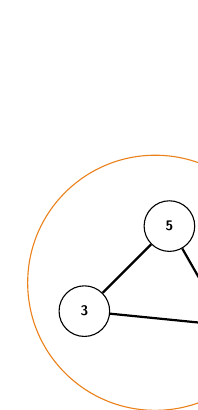
\begin{tikzpicture}[scale=1.8,auto,swap]

            \node[vertex] (1) at (-0.8,1.9) {1};
            \node[vertex] (2) at (3,1.7) {2};
            \node[vertex] (3) at (0.4,0.5) {3};
            \node[vertex] (4) at (-1.2,1.2) {4};
            \node[vertex] (5) at (1,1.1) {5};
            \node[vertex] (6) at (1.4,0.4) {6};
            \node[vertex] (7) at (-1.9,1.7) {7};

            \path[edge] (1) -- (4);
            \path[edge] (4) -- (7);
            \path[edge] (3) -- (5);
            \path[edge] (5) -- (6);
            \path[edge] (6) -- (3);

            \onslide<3->{
                \draw[color=vhilight] (-1.3,1.55) ellipse (0.9cm and 0.9cm);
                \draw[color=vhilight] (0.9,0.7) ellipse (0.9cm and 0.9cm);
                \draw[color=vhilight] (3,1.7) ellipse (0.3cm and 0.3cm);
            }

            \pgfresetboundingbox
            \path [use as bounding box] (0,0) rectangle (1,2.5);
        \end{tikzpicture}
    \end{figure}

    \bi
        \onslide<2->{\item $elementos = \{1,2,3,4,5,6,7\}$}
        \onslide<3->{\item $colecciones = \{1,4,7\}, \{2\}, \{3,5,6\}$}
        \onslide<4->{\item \texttt{union(2, 5)}}
    \ei
\end{frame}


\begin{frame}{Conjuntos disjuntos en grafos}
    \begin{figure}
        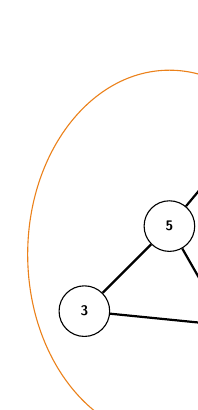
\begin{tikzpicture}[scale=1.8,auto,swap]

            \node[vertex] (1) at (-0.8,1.9) {1};
            \node[vertex] (2) at (1.5,1.7) {2};
            \node[vertex] (3) at (0.4,0.5) {3};
            \node[vertex] (4) at (-1.2,1.2) {4};
            \node[vertex] (5) at (1,1.1) {5};
            \node[vertex] (6) at (1.4,0.4) {6};
            \node[vertex] (7) at (-1.9,1.7) {7};

            \path[edge] (1) -- (4);
            \path[edge] (4) -- (7);
            \path[edge] (3) -- (5);
            \path[edge] (5) -- (6);
            \path[edge] (6) -- (3);
            \path[edge] (2) -- (5);

            \draw[color=vhilight] (-1.3,1.55) ellipse (0.9cm and 0.9cm);
            \draw[color=vhilight] (1.0,0.9) ellipse (1.0cm and 1.3cm);

            \pgfresetboundingbox
            \path [use as bounding box] (0,0) rectangle (1,2.5);
        \end{tikzpicture}
    \end{figure}

    \bi
        \item $elementos = \{1,2,3,4,5,6,7\}$
        \item $colecciones = \{1,4,7\}, \{2,3,5,6\}$
        \onslide<2->{\item \texttt{union(6, 2)}}
    \ei
\end{frame}


\begin{frame}{Conjuntos disjuntos en grafos}
    \begin{figure}
        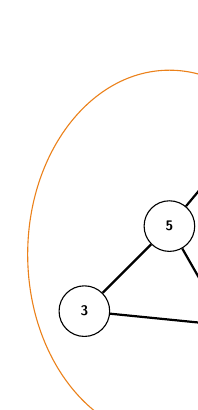
\begin{tikzpicture}[scale=1.8,auto,swap]

            \node[vertex] (1) at (-0.8,1.9) {1};
            \node[vertex] (2) at (1.5,1.7) {2};
            \node[vertex] (3) at (0.4,0.5) {3};
            \node[vertex] (4) at (-1.2,1.2) {4};
            \node[vertex] (5) at (1,1.1) {5};
            \node[vertex] (6) at (1.4,0.4) {6};
            \node[vertex] (7) at (-1.9,1.7) {7};

            \path[edge] (1) -- (4);
            \path[edge] (4) -- (7);
            \path[edge] (3) -- (5);
            \path[edge] (5) -- (6);
            \path[edge] (6) -- (3);
            \path[edge] (2) -- (5);
            \path[edge] (2) -- (6);

            \draw[color=vhilight] (-1.3,1.55) ellipse (0.9cm and 0.9cm);
            \draw[color=vhilight] (1.0,0.9) ellipse (1.0cm and 1.3cm);

            \pgfresetboundingbox
            \path [use as bounding box] (0,0) rectangle (1,2.5);
        \end{tikzpicture}
    \end{figure}

    \bi
        \item $elementos = \{1,2,3,4,5,6,7\}$
        \item $colecciones = \{1,4,7\}, \{2,3,5,6\}$
    \ei
\end{frame}

\begin{frame}{Problema de ejemplo: Where's My Internet??}
    \bi
        \item \href{https://open.kattis.com/problems/wheresmyinternet}{https://open.kattis.com/problems/wheresmyinternet}
    \ei
\end{frame}

\begin{frame}{Problema de ejemplo: Where's My Internet??}

  \begin{block}{Descripcion del problema}
    En una ciudad hay $n$ casas y algunas no tienen conexión a internet. 
    
    Las casas están numeradas de $1$ a $n$. 
    La casa $1$ ya tiene conexión a internet a través de un cable que va a otra ciudad. 
    Una casa tiene conexión a internet si tiene un cable a otra casa que ya está conectada a internet.

    Dada una lista de pares de casas que ya están conectadas, indicar los números de las casas que no tienen conexión a internet.
    \end{block}
\end{frame}

\begin{frame}{Problema de ejemplo: Where's My Internet??}
  \begin{block}{Input}
    La primera línea contiene dos enteros $n$ y $m$, el número de casas y el número de pares de casas que ya están conectadas.
    Las siguientes $m$ líneas contienen dos enteros $a_i$, $b_i$ indicando que las casas $a_i$ y $b_i$ ya están conectadas.
    \end{block}

    \vspace{10pt}

    \begin{block}{Output}
    Si todas las casas tienen conexión a internet, imprimir ``\texttt{Connected}''.

    Si no, imprimir una línea por cada casa que no tiene conexión a internet, en orden ascendente.
    \end{block}
\end{frame}

\begin{frame}{Problema de ejemplo: Where's My Internet??}
  \begin{center}
    \begin{tabular}{|l|l|}
        \hline
        {\footnotesize Input de ejemplo} & {\footnotesize Output de ejemplo} \\
        \hline
        \begin{minipage}{80pt}
\vspace{10pt}
\ttfamily
6 4 \\
1 2 \\
2 3 \\
3 4 \\
5 6 \\
        \end{minipage}
&
\begin{minipage}{80pt}
\vspace{10pt}
\ttfamily
5 \\
6 \\
\end{minipage}
\\
        \hline
    \end{tabular}
\end{center}
\end{frame}

\begin{frame}[fragile]{Problema de ejemplo: Where's My Internet??}
  \begin{minted}{cpp}
  int p[MAXN];
  int find(int x) {...}
  void unite(int x, int y) {...}

  int main() {
    int n, m;
    cin >> n >> m;
    for (int i = 1; i <= n; ++i) p[i] = i;
    for (int i = 0; i < m; ++i) {
      int a, b;
      cin >> a >> b;
      unite(a, b);
    }
    // encontrar casas no conectadas
  }
  \end{minted}
\end{frame}

\begin{frame}[fragile]{Problema de ejemplo: Where's My Internet??}
  \begin{minted}{cpp}
    // encontrar casas no conectadas
    bool connected = true;
    for (int i = 1; i <= n; ++i) {
      if (find(1) != find(i)) {
        cout << i << endl;
        connected = false;
      }
    }
    if (connected) {
      cout << "Connected" << endl;
    }
  \end{minted}
\end{frame}

\begin{frame}{Almacenar información sobre el conjunto}
  \bi
    \item A veces no solo queremos saber si dos elementos están en el mismo conjunto
    \item ¿Cuántos elementos hay en el conjunto?
    \item ¿Cuál es el elemento más pequeño del conjunto?
    
    \vspace{20pt}

    \item<2-> Podemos almacenar esta información en el elemento representativo del conjunto
    \item<2-> Debemos tener cuidado al actualizar esta información cuando unimos dos conjuntos
  \ei
\end{frame}

\begin{frame}{Almacenar información sobre el conjunto}
  \begin{figure}
    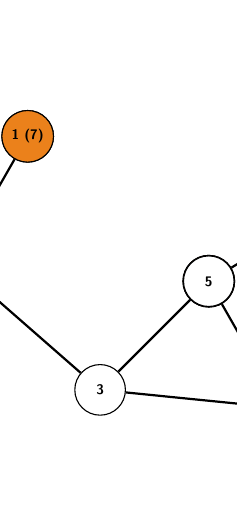
\begin{tikzpicture}[scale=2.3,auto,swap]

        \node[vertex, fill=vhilight] (1) at (0,1.9) {1 (3)};
        \node[vertex, fill=vhilight] (2) at (2,1.7) {};
        \node[vertex] (3) at (0.4,0.5) {3};
        \node[vertex] (4) at (-0.4,1.2) {4};
        \node[vertex, fill=vhilight] (5) at (1,1.1) {5 (3)};
        \node[vertex] (6) at (1.4,0.4) {6};
        \node[vertex] (7) at (-1,1.7) {7};

        \path[edge] (1) -- (4);
        \path[edge] (4) -- (7);
        \path[edge] (3) -- (5);
        \path[edge] (5) -- (6);
        \path[edge] (6) -- (3);
        
        \onslide<1>{
          \node[vertex, fill=vhilight] (2) at (2) {2 (1)};
        }
        \onslide<2->{
          \node[vertex, fill=vhilight] (5) at (5) {5 (4)};
          \node[vertex, fill=white] (2) at (2) {2};
          \path[edge] (2) -- (5);
        }
        \onslide<4->{
          \node[vertex, fill=vhilight] (1) at (1) {1 (7)};
          \node[vertex, fill=white] (5) at (5) {5};
          \path[edge] (4) -- (3);
        }

        \pgfresetboundingbox
        \path [use as bounding box] (0,0) rectangle (1,2.5);
    \end{tikzpicture}
  \end{figure}

  \bi
    \item<2-> \texttt{union(2, 5)}
    \item<3-> \texttt{union(3, 4)}
  \ei
\end{frame}

\begin{frame}[fragile]{Almacenar información sobre el conjunto}
  \begin{minted}{cpp}
  int p[MAXN], sz[MAXN];
  int find(int x) {...}
  void unite(int x, int y) {
    x = find(x);
    y = find(y);
    // para no actualizar con información duplicada
    if (x == y) return; 

    p[y] = x;
    sz[x] += sz[y];
  }
  // sz[find(x)] <- tamaño del conjunto de x
  \end{minted}
\end{frame}

\begin{frame}[fragile]{Almacenar información sobre el conjunto}
  \begin{minted}{cpp}
  int p[MAXN], sz[MAXN];
  int find(int x) {...}
  void unite(int x, int y) {
    x = find(x);
    y = find(y);
    // para no actualizar con información duplicada
    if (x == y) return; 
    if (sz[x] < sz[y]) swap(x, y); // O(1) en practica
    p[y] = x;
    sz[x] += sz[y];
  }
  // sz[find(x)] <- tamaño del conjunto de x
  \end{minted}
\end{frame}

\end{document}

